% Frozen exploratory canonicalization-phase times that the Tier 1 replay tests.
% Data: ../../packed_index_e1_canonical_20261009/run_{1..6}_*.json, timing_ns.target_cycle_canonical.
% Source of figures/exploratory_phases.pdf; build: pdflatex exploratory_phases.tex
\documentclass[border=6pt]{standalone}
\usepackage{pgfplots}
\pgfplotsset{compat=1.17}
\begin{document}
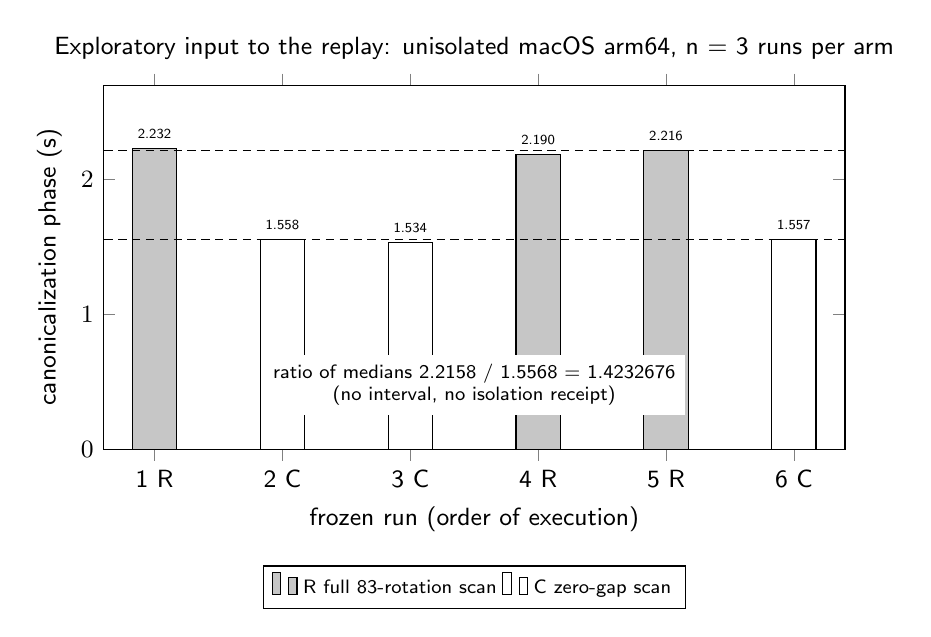
\begin{tikzpicture}[font=\sffamily\small]
\begin{axis}[width=11cm, height=6.2cm, ybar, bar width=16pt, bar shift=0pt, ymin=0, ymax=2.7, enlarge x limits=0.08,
  ylabel={canonicalization phase (s)}, xlabel={frozen run (order of execution)},
  xtick={1,2,3,4,5,6}, xticklabels={1 R,2 C,3 C,4 R,5 R,6 C},
  title={Exploratory input to the replay: unisolated macOS arm64, n = 3 runs per arm},
  title style={font=\sffamily\small}, legend style={at={(0.5,-0.32)}, anchor=north, legend columns=2, font=\sffamily\scriptsize},
  nodes near coords, every node near coord/.append style={font=\sffamily\tiny}, point meta=explicit symbolic]
\addplot[fill=gray!45, draw=black] coordinates {(1,2.231706) [2.232] (4,2.190246) [2.190] (5,2.215795) [2.216]};
\addplot[fill=white, draw=black] coordinates {(2,1.557506) [1.558] (3,1.534029) [1.534] (6,1.556837) [1.557]};
\draw[densely dashed] (axis cs:0.5,2.215795) -- (axis cs:6.5,2.215795);
\draw[densely dashed] (axis cs:0.5,1.556837) -- (axis cs:6.5,1.556837);
\node[anchor=south, font=\sffamily\scriptsize, fill=white, align=center] at (axis cs:3.5,0.25) {ratio of medians 2.2158 / 1.5568 = 1.4232676\\(no interval, no isolation receipt)};
\legend{R full 83-rotation scan, C zero-gap scan}
\end{axis}
\end{tikzpicture}
\end{document}
